\documentclass[border=0.2cm]{standalone}

% Required package and libraries
\usepackage{tikz}
\usetikzlibrary{decorations.pathmorphing,patterns}

\begin{document}

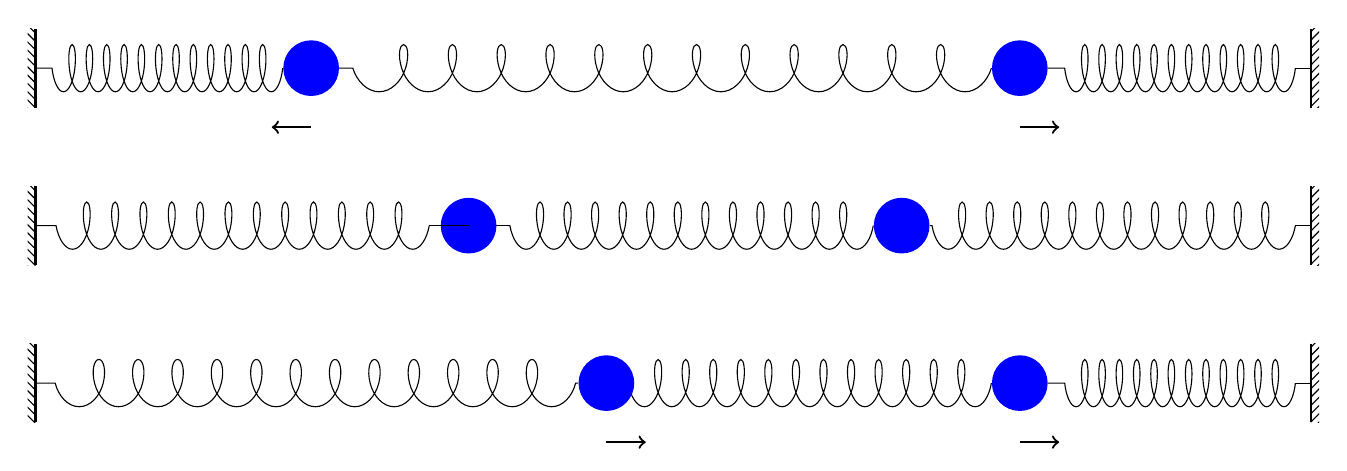
\begin{tikzpicture}


%grid help
% \draw[gray, very thin] (-12,-4) grid (7,2);


% Left Supporting structure
		\fill [pattern = north west lines] (-11.1,-.50) rectangle (-11.0,.5);
		\draw[thick] (-11.0,-.50) -- (-11.0,.50);

%Mass
\node[circle,fill=blue,inner sep=2.5mm] (a) at (0,0) {};

%Spring on the right
\draw[decoration={aspect=0.4, segment length=3.5mm, amplitude=3mm,coil},decorate] (5,0) -- (a); 
\draw[] (5.0,0) -- (5.2,0);
%Spring in the middle
%%\draw[decoration={aspect=0.3, segment length=3mm, amplitude=3mm,coil},decorate] (-5,0) -- (a); 
\draw[decoration={aspect=0.4, segment length=3.5mm, amplitude=3mm,coil},decorate] (a) -- (-5,0); 
\draw[] (-5.5,0) -- (-5.0,0);
%Mass
\node[circle,fill=blue,inner sep=2.5mm] (b) at (-5.5,0) {};

%Spring on the left (segment length doesn't match, but gets correct number of coils)
\draw[decoration={aspect=0.4, segment length=3.6mm, amplitude=3mm,coil},decorate] (-6.0,0) -- (-11,0); 
\draw[] (-6.0,0) -- (-5.5,0);

% Right Supporting structure
		\fill [pattern = north east lines] (5.2,-.50) rectangle (5.3,.5);
		\draw[thick] (5.20,-.50) -- (5.20,.50);

%%%%%%%%%%%% Second pattern %%%%%%%%%%%%%%%%%%%

% Left Supporting structure
		\fill [pattern = north west lines] (-11.1,1.50) rectangle (-11,2.5);
		\draw[thick] (-11.0,1.50) -- (-11.0,2.50);

%Mass
\node[circle,fill=blue,inner sep=2.5mm] (c) at (1.5,2.0) {};
% Draw the arrow underneath the circle
    \draw[->, thick] (1.5,1.25) -- (2.0,1.25);

%Spring on the right
\draw[decoration={aspect=0.3, segment length=2.2mm, amplitude=3mm,coil},decorate] (5,2.) -- (c); 
\draw[] (5.0,2.0) -- (5.2,2.0);
%Spring in the middle
%%\draw[decoration={aspect=0.3, segment length=3mm, amplitude=3mm,coil},decorate] (-5,0) -- (a); 
\draw[decoration={aspect=0.6, segment length=6.2mm, amplitude=3mm,coil},decorate] (c) -- (-7.5,2.0); 
%\draw[] (-6.0,2.0) -- (-6.2,2.0);
%Mass
\node[circle,fill=blue,inner sep=2.5mm] (b) at (-7.5,2.0) {};
% Draw the arrow underneath the circle
    \draw[->, thick] (-7.5,1.25) -- (-8.0,1.25);

%Spring on the left
%%\draw[decoration={aspect=0.3, segment length=2.4mm, amplitude=3mm,coil},decorate] (-6.3,2.0) -- (-11,2.0); 
\draw[decoration={aspect=0.3, segment length=2.2mm, amplitude=3mm,coil},decorate] (b) -- (-11,2.0);

%\draw[] (-6.0,0) -- (-5.5,0);

% Right Supporting structure
		\fill [pattern = north east lines] (5.2,1.50) rectangle (5.3,2.5);
		\draw[thick] (5.20,1.50) -- (5.20,2.50);

%%%%%%%%%%%% Third pattern %%%%%%%%%%%%%%%%%%%

% Left Supporting structure
		\fill [pattern = north west lines] (-11.1,-1.50) rectangle (-11,-2.5);
		\draw[thick] (-11.0,-1.50) -- (-11.0,-2.50);

%Mass
\node[circle,fill=blue,inner sep=2.5mm] (c) at (1.5,-2.0) {};
% Draw the arrow underneath the circle
    \draw[->, thick] (1.5,-2.75) -- (2.0,-2.75);
    
%Spring on the right
\draw[decoration={aspect=0.3, segment length=2.2mm, amplitude=3mm,coil, post length=0.5mm},decorate] (5,-2.) -- (c); 
\draw[] (5.0,-2.0) -- (5.2,-2.0);


%Spring in the middle
%%\draw[decoration={aspect=0.3, segment length=3mm, amplitude=3mm,coil},decorate] (-5,0) -- (a); 
\draw[decoration={aspect=0.4, segment length=3.5mm, amplitude=3mm,coil},decorate] (c) -- (-3.5,-2.0); 
%\draw[] (-6.0,2.0) -- (-6.2,2.0);
%Mass
\node[circle,fill=blue,inner sep=2.5mm] (b) at (-3.75,-2.0) {};
% Draw the arrow underneath the circle
    \draw[->, thick] (-3.75,-2.75) -- (-3.25,-2.75);


%Spring on the left
%%\draw[decoration={aspect=0.3, segment length=2.4mm, amplitude=3mm,coil},decorate] (-6.3,2.0) -- (-11,2.0); 
\draw[decoration={aspect=0.6, segment length=5.0mm, amplitude=3mm,coil, pre length=0.3mm},decorate] (b) -- (-11,-2.0);

%\draw[] (-6.0,0) -- (-5.5,0);

% Right Supporting structure
		\fill [pattern = north east lines] (5.2,-1.50) rectangle (5.3,-2.5);
		\draw[thick] (5.20,-1.50) -- (5.20,-2.50);





\end{tikzpicture}	
\end{document}
